\documentclass{article}
\usepackage{tikz}
\usetikzlibrary{positioning,arrows.meta}  % Use arrows.meta for arrow styles

\begin{document}

% Slide 4: RNN Structures
\section*{RNN Structures}
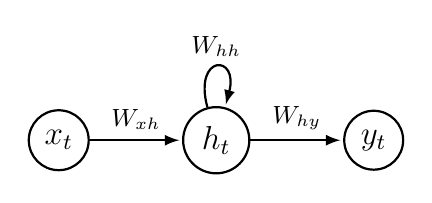
\begin{tikzpicture}[->,>=latex,shorten >=1pt,auto,node distance=2cm,  % Changed 'stealth' to 'latex'
  thick,main node/.style={circle,draw,font=\sffamily\large\bfseries}]
  \node[main node] (1) {$x_{t}$};
  \node[main node] (2) [right of=1] {$h_{t}$};
  \node[main node] (3) [right of=2] {$y_{t}$};
  
  \path[every node/.style={font=\sffamily\small}]
    (1) edge node [above] {$W_{xh}$} (2)
    (2) edge node [above] {$W_{hy}$} (3)
    (2) edge [loop above] node [above] {$W_{hh}$} (2);
\end{tikzpicture}

% Slide 5: Working Principle of RNNs
\section*{Working Principle of RNNs}
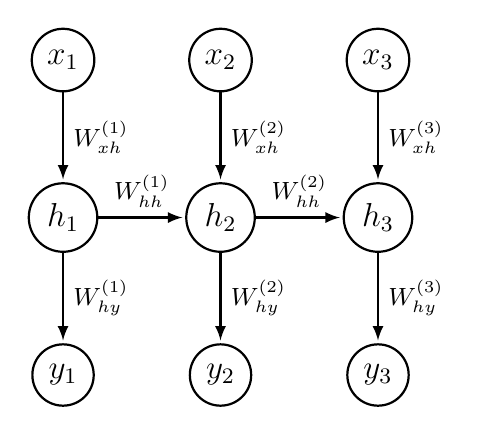
\begin{tikzpicture}[->,>=latex,shorten >=1pt,auto,node distance=2cm,
  thick,main node/.style={circle,draw,font=\sffamily\large\bfseries}]
  
  \node[main node] (x1) {$x_{1}$};
  \node[main node] (x2) [right of=x1] {$x_{2}$};
  \node[main node] (x3) [right of=x2] {$x_{3}$};
  
  \node[main node] (h1) [below of=x1] {$h_{1}$};
  \node[main node] (h2) [below of=x2] {$h_{2}$};
  \node[main node] (h3) [below of=x3] {$h_{3}$};
  
  \node[main node] (y1) [below of=h1] {$y_{1}$};
  \node[main node] (y2) [below of=h2] {$y_{2}$};
  \node[main node] (y3) [below of=h3] {$y_{3}$};
  
  \path[every node/.style={font=\sffamily\small}]
    (x1) edge node [right] {$W_{xh}^{(1)}$} (h1)
    (x2) edge node [right] {$W_{xh}^{(2)}$} (h2)
    (x3) edge node [right] {$W_{xh}^{(3)}$} (h3)
    (h1) edge node [right] {$W_{hy}^{(1)}$} (y1)
    (h2) edge node [right] {$W_{hy}^{(2)}$} (y2)
    (h3) edge node [right] {$W_{hy}^{(3)}$} (y3)
    (h1) edge node [above] {$W_{hh}^{(1)}$} (h2)
    (h2) edge node [above] {$W_{hh}^{(2)}$} (h3);
\end{tikzpicture}

% Slide 9: Stacked RNNs
\section*{Stacked RNNs}
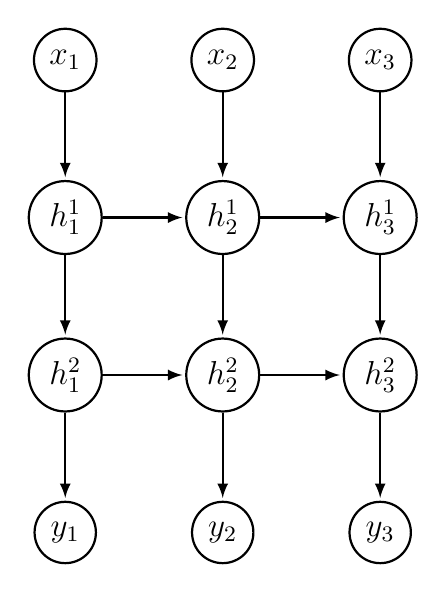
\begin{tikzpicture}[->,>=latex,shorten >=1pt,auto,node distance=2cm,
  thick,main node/.style={circle,draw,font=\sffamily\large\bfseries}]
  
  \node[main node] (x1) {$x_{1}$};
  \node[main node] (x2) [right of=x1] {$x_{2}$};
  \node[main node] (x3) [right of=x2] {$x_{3}$};
  
  \node[main node] (h11) [below of=x1] {$h_{1}^{1}$};
  \node[main node] (h12) [below of=x2] {$h_{2}^{1}$};
  \node[main node] (h13) [below of=x3] {$h_{3}^{1}$};
  
  \node[main node] (h21) [below of=h11] {$h_{1}^{2}$};
  \node[main node] (h22) [below of=h12] {$h_{2}^{2}$};
  \node[main node] (h23) [below of=h13] {$h_{3}^{2}$};
  
  \node[main node] (y1) [below of=h21] {$y_{1}$};
  \node[main node] (y2) [below of=h22] {$y_{2}$};
  \node[main node] (y3) [below of=h23] {$y_{3}$};
  
  \path[every node/.style={font=\sffamily\small}]
    (x1) edge (h11)
    (x2) edge (h12)
    (x3) edge (h13)
    (h11) edge (h21)
    (h12) edge (h22)
    (h13) edge (h23)
    (h21) edge (y1)
    (h22) edge (y2)
    (h23) edge (y3)
    (h11) edge (h12)
    (h12) edge (h13)
    (h21) edge (h22)
    (h22) edge (h23);
\end{tikzpicture}

% Slide 10: Bidirectional RNNs
\section*{Bidirectional RNNs}
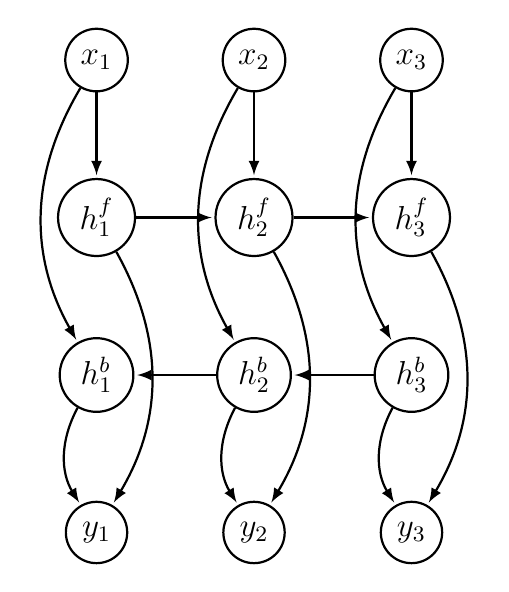
\begin{tikzpicture}[->,>=latex,shorten >=1pt,auto,node distance=2cm,
  thick,main node/.style={circle,draw,font=\sffamily\large\bfseries}]
  
  \node[main node] (x1) {$x_{1}$};
  \node[main node] (x2) [right of=x1] {$x_{2}$};
  \node[main node] (x3) [right of=x2] {$x_{3}$};
  
  \node[main node] (hf1) [below of=x1] {$h_{1}^{f}$};
  \node[main node] (hf2) [below of=x2] {$h_{2}^{f}$};
  \node[main node] (hf3) [below of=x3] {$h_{3}^{f}$};
  
  \node[main node] (hb1) [below of=hf1] {$h_{1}^{b}$};
  \node[main node] (hb2) [below of=hf2] {$h_{2}^{b}$};
  \node[main node] (hb3) [below of=hf3] {$h_{3}^{b}$};
  
  \node[main node] (y1) [below of=hb1] {$y_{1}$};
  \node[main node] (y2) [below of=hb2] {$y_{2}$};
  \node[main node] (y3) [below of=hb3] {$y_{3}$};
  
  \path[every node/.style={font=\sffamily\small}]
    (x1) edge (hf1)
    (x2) edge (hf2)
    (x3) edge (hf3)
    (x3) edge [bend right] (hb3)
    (x2) edge [bend right] (hb2)
    (x1) edge [bend right] (hb1)
    (hf1) edge (hf2)
    (hf2) edge (hf3)
    (hb3) edge (hb2)
    (hb2) edge (hb1)
    (hf1) edge [bend left] (y1)
    (hb1) edge [bend right] (y1)
    (hf2) edge [bend left] (y2)
    (hb2) edge [bend right] (y2)
    (hf3) edge [bend left] (y3)
    (hb3) edge [bend right] (y3);
\end{tikzpicture}

\end{document}
